\subsection{Initialization}

Before processing queries, \Natural~requires initialization with reference
data to construct an embedding space $v \in \mathcal{V}$ and schema distance
index $d \in \mathcal{D}$. This preprocessing phase analyzes datasets and
previous user interactions to enable schema-aware example selection.

The initialization process consists of two components: (1) embedding generation
for semantic similarity computation, and (2) schema indexing for structural
similarity measurement. These components support the example selection function
$\sigma$.

\subsubsection{Embedding}\label{design:embedding}

\textsc{Natural} constructs an embedding space $v$ to enable semantic
similarity search \citep{DAIL-SQL}. It uses cosine similarity to identify
relevant examples based on natural language queries and SQL statements,
allowing efficient retrieval from large collections of question-answer pairs.

Therefore a set of training samples can be embedded $\mathcal{T} = \{(q_1,
\omega_1), ..., (q_n, \omega_n)\}$ into an embedding space $v$, where each
$q_i$ is a natural language question and $\omega_i$ is the corresponding SQL
query.

The embedding space $v$ can be formally defined as:

$$v = \{~(q, \iota(q), \omega, \iota(\omega))~|~(q, \omega) \in \mathcal{T}~\}$$

where $\iota$ is the embedding function that maps text to vector representations.

\subsubsection{Schema Indexing}

To choose relevant samples for ICL, the SQL queries chosen as examples should
use structurally similar database schemas to minimize the structural difference
between the selected samples and the ground truth query for a natural language
question.

For example $\omega_{ground}$ the question ``Give me all contacts for the user
with the id 10'' might look different depending on the database schema, thus
selecting samples based only on the similarity of the natural language question
will yield inferior sample quality.

\begin{figure}[ht]
  \vspace{1em}
  \hfill
  \begin{minipage}[b]{0.40\linewidth}
    \begin{verbatim}
CREATE TABLE users (
  id TEXT PRIMARY KEY
);

CREATE TABLE contacts (
  user_id TEXT NOT NULL,
  name TEXT NOT NULL,
  FOREIGN KEY (user_id) 
   REFERENCES users(id),
  PRIMARY KEY (user_id, name)
);
    \end{verbatim}
    \caption{Normalized SQL database schema with separate tables for users and contacts.}
    \label{figure:schema-normalized}
  \end{minipage}
  \hfill
  \begin{minipage}[b]{0.4\linewidth}
    \begin{verbatim}
CREATE TABLE users (
  id TEXT PRIMARY KEY,
  contacts TEXT[] NOT NULL
);
    \end{verbatim}
    \vspace{3.75em}
    \caption{Denormalized SQL database schema with contacts stored within an array column.}
    \label{figure:schema-denormalized}
  \end{minipage}
  \hfill
  \vspace{1em}
\end{figure}

Given the database schemas in Figures~\ref{figure:schema-normalized}
and~\ref{figure:schema-denormalized} respective definitions of
$\omega_{ground}$ would be~\ref{figure:sql-join-example}
and~\ref{figure:sql-array-example}.

\begin{figure}[ht]
  \vspace{1em}
  \hfill
  \begin{minipage}[b]{0.4\linewidth}
    \begin{verbatim}
SELECT contacts.name
FROM users
JOIN contacts
  ON contacts.user_id = users.id
WHERE users.id = 10;
    \end{verbatim}
    \caption{Using JOIN on a normalized database schema in SQL.}
    \label{figure:sql-join-example}
  \end{minipage}
  \hfill
  \begin{minipage}[b]{0.4\linewidth}
    \centering
    \begin{verbatim}
SELECT contacts
FROM users
WHERE id = 10;
    \end{verbatim}
    \vspace{1.3em}
    \caption{Using array access on a denormalized database schemas in SQL.}
    \label{figure:sql-array-example}
  \end{minipage}
  \hfill
  \vspace{1em}
\end{figure}


Figures~\ref{figure:sql-join-example} and~\ref{figure:sql-array-example} show
the structural similarity of the database schema is crucial to
the relevance of an example.

\paragraph{Graph Representation}\label{design:graph-repr}

To determine structural similarity of database schemas, this thesis proposes
using graph representation for the representation of database structures. A
graph representation allows leveraging established methods for measuring graph
similarity such as Wasserstein-Weisfeiler-Lehman graph kernels \citep{WWL}. 
Given a database schema $s$ the corresponding graph mapping $G_s = (V, E, \ell,
w)$ is defined in Tables~\ref{table:nodes} and~\ref{table:edges}.

\begin{table}[ht]
  \hfill
  \begin{minipage}[b]{0.45\linewidth}
    \centering
    \begin{tabular}{clc}
      \hline
      \textbf{Node Type} & \textbf{Description} & \textbf{Label $\ell(v)$} \\
      \hline
      $v \in V_t$ & Tables & 1 \\
      $v \in V_c$ & Generic columns & 2 \\
      $v \in V_c$ & Primary keys & 3 \\
      $v \in V_c$ & Foreign keys & 4 \\
      $v \in V_c$ & Text columns  & 5 \\
      $v \in V_c$ & Numeric columns & 6 \\
      $v \in V_c$ & Datetime columns & 7 \\
      $v \in V_c$ & Boolean columns & 8 \\
      $v \in V_c$ & Other columns & 9 \\
      \hline
    \end{tabular}
    \caption{
      Node types and semantic labels where $V = V_t \cup V_c$ where $V_t$ represents
      table nodes and $V_c$ represents column nodes
    }
    \label{table:nodes}
  \end{minipage}
  \hfill
  \begin{minipage}[b]{0.45\linewidth}
    \centering
    \begin{tabular}{clc}
      \hline
      \textbf{Edge Type} & \textbf{Description} & \textbf{Weight $w(e)$} \\
      \hline
      $e \in E_{tc}$ & Ownership & 0.5 \\
      $e \in E_{fk}$ & FK references & 0.9 \\
      $e \in E_{rel}$ & Relationships & 1.0 \\
      \hline
    \end{tabular}
    \vspace{3.5em}
    \caption{Edge types and weights where $E = E_{tc} \cup E_{fk} \cup E_{rel}$}
    \label{table:edges}
    \vspace{1em}
  \end{minipage}
  \hfill
  \vspace{1em}
\end{table}


The structural similarity of two databases is defined as the wasserstein
distance of their graphs. The graph representation captures essential
topology through node and edge labeling, prioritizing constraints over
types. This hierarchical labeling ensures that structural relationships
take precedence over exact content, while omitting table names, column names
and domain terminology for schema-agnostic comparison.
The graph representation of the database schemas introduced
in~\ref{figure:schema-normalized} and~\ref{figure:schema-denormalized} are
therefore:

\begin{figure}[ht]
  \vspace{1em}
  \hfill
  \begin{minipage}[b]{0.45\linewidth}
    \centering
    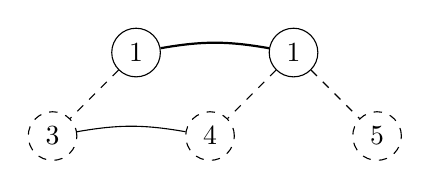
\begin{tikzpicture}[node distance={15mm}, table/.style = {draw,circle}, column/.style = {draw,dashed,circle}]

      \node[table] (users) at (0,0) {1}; 
      \node[table] (contacts) at (2,0) {1}; 
      
      \node[column] (users_id) [below left of=users] {3}; 
      
      \node[column] (contacts_user_id) [below left of=contacts] {4};
      \node[column] (contacts_name) [below right of=contacts] {5};
      
      \draw[dashed] (users) -- (users_id); 
      \draw[dashed] (contacts) -- (contacts_user_id); 
      \draw[dashed] (contacts) -- (contacts_name); 
      
      \draw[thick] (users) to [out=10, in=170] (contacts);
      
      \draw (users_id) to [out=10, in=170] (contacts_user_id); 
    \end{tikzpicture} 
    \caption{Graph representation of a normalized schema.}
    \label{figure:normalized-graph-representation}
  \end{minipage}
  \hfill
  \begin{minipage}[b]{0.45\linewidth}
    \centering
    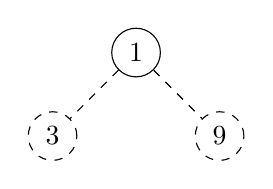
\begin{tikzpicture}[node distance={15mm}, table/.style = {draw,circle}, column/.style = {draw,dashed,circle}]
      \node[table] (users) at (0,0) {1}; 
      
      \node[column] (users_id) [below left of=users] {3}; 
      \node[column] (users_contacts) [below right of=users] {9};
      
      \draw[dashed] (users) -- (users_id); 
      \draw[dashed] (users) -- (users_contacts); 
    \end{tikzpicture} 
    \caption{Graph representation of a denormalized schema.}
    \label{figure:denormalized-graph-representation}
  \end{minipage}
  \hfill
  \vspace{1em}
  
  \begin{minipage}{\linewidth}
    \centering
    \vspace{0.5em}
    \small
    \textbf{Legend:} \cir{}~table~~\cir{dashed}~column~~\textbf{-}~foreign key~~--~reference~~- -~table-column
  \end{minipage}
\end{figure}

The $\Delta$ of the order of the
graphs~\ref{figure:normalized-graph-representation}
and~\ref{figure:denormalized-graph-representation} further highlight the
structural difference between the two schemas.

\paragraph{Distance Measurement}

To measure the distance between the graphs shown
in Figures~\ref{figure:normalized-graph-representation}
and~\ref{figure:denormalized-graph-representation}, the Wasserstein
Weisfeiler-Lehman (WWL) graph kernel method is used \citep{WWL}. WWL kernels
compute structural similarity by combining discrete Weisfeiler-Lehman graph
features with continuous optimal transport theory. The method first extracts WL
features from the labeled graph structure, then computes the Wasserstein
distance between the resulting feature distributions. For two graphs $G$ and
$G'$ with semantic node labels, the distance is computed as introduced by
\citeauthor{WWL} in \citeyear{WWL}:

\begin{equation}
D^{f}_{W}(G, G') = W_1(f(G), f(G'))
\end{equation}

The graph representation of the normalized schema $G_{norm}$ (see
Figure~\ref{figure:normalized-graph-representation}) with 5 nodes and 5 edges
and denormalized schema $G_{denorm}$ (see
Figure~\ref{figure:denormalized-graph-representation}) with 3 nodes and 2 edges
show significant topological differences. The WWL distance measures the
reduced graph complexity (i.e., fewer nodes and edges) and the loss of
relational structure (i.e., elimination of foreign key relationships),
which results in a higher distance measurement despite modeling logically
equivalent data: $D^{f}_{W}(G_{norm}, G_{denorm}) \approx 0.78$.

\paragraph{Distance Index}

The distance index $d$ contains precomputed distances between observed the
database schemas, which enables an efficient retrieval during example
selection. This index is constructed as a set of schema-distance tuples
$\{(sm_1, di_1), \ldots, (sm_i, di_i)\}$ where $sm_i$ is a database schema name
and $di_i$ denotes its WWL distance to the current schema.
